\section{高阶微分与极值判别}
\label{sec:multivariable-curvature-error}

一阶微分用切平面描述局部变化，却看不出曲面向哪边弯：碗底、山顶和马鞍点处的切平面都是水平的。切平面遗漏的部分中，最先出现的是弯曲。把第~\ref{sec:multivariable-vector-differentiation}节的向量值微分用于梯度映射，就能研究一阶变化本身怎样变化，从而描述弯曲。

前面已建立的多线性映射、二次型和谱判别，在这里分别用于表示高阶导数、衡量二阶项和判断局部形状。本节先把二阶偏导数集中为Hessian矩阵并解释为二阶微分，再借一元Taylor公式建立二阶近似，最后据此判断驻点的类型。

\subsection{二阶偏导数、Hessian与高阶微分}

一阶偏导数本身仍是多元标量函数，可以再求偏导。这里记$f_{x_i x_j}=\partial_j(\partial_i f)$，即先对$x_i$、再对$x_j$求导。
$f_{xx}$描述$x$方向切片的斜率沿$x$方向怎样变化，即该切片的弯曲。混合偏导数$f_{xy}$描述沿$y$方向移动时$x$方向的斜率怎样变化，即曲面的扭转。

对$f(x,y)=x^2+xy+y^2$，二阶偏导数为
\[
 f_{xx}=2,\qquad f_{xy}=f_{yx}=1,\qquad f_{yy}=2.
\]

又如$f(x,y)=xy$：$x$方向切片的斜率是$y$，向北每走一单位，这个斜率就增加$1$，故$f_{xy}=1$，而$f_{xx}=f_{yy}=0$。它的每条坐标切片都是直线，曲面却是扭曲的。
这两个例子中都有$f_{xy}=f_{yx}$。一般函数的混合偏导数能否交换次序，则需要额外条件。

\paragraph{混合偏导数的交换}
先看一个反例：两个次序的混合偏导数都存在，却不相等。
\begin{example}[混合偏导数与求导次序有关]
\label{ex:multivariable-mixed-partials-differ}
令$f(0,0)=0$，非原点处令
\[
 f(x,y)=\frac{xy(x^2-y^2)}{x^2+y^2}.
\]
对$y\neq0$，因为$f(0,y)=0$，
\[
 \begin{aligned}
 f_x(0,y)&=\lim_{h\to0}\frac{f(h,y)}h\\
 &=\lim_{h\to0}\frac{y(h^2-y^2)}{h^2+y^2}=-y;
 \end{aligned}
\]
又$f$在$x$轴上恒为$0$，故$f_x(0,0)=0$，公式$f_x(0,y)=-y$在$y=0$时也成立。同样算得$f_y(x,0)=x$对所有$x$成立。于是
\[
 \begin{gathered}
f_{xy}(0,0)=\frac{\mathrm d}{\mathrm dy}(-y)\Big|_{y=0}=-1\\
f_{yx}(0,0)=\frac{\mathrm d}{\mathrm dx}x\Big|_{x=0}=1,
 \end{gathered}
\]
两个次序给出不同结果。
\end{example}

下面的定理说明，混合偏导数在基点连续时两种次序一定相同。因此本例的混合偏导数不可能都在原点连续。
\begin{theorem}[混合偏导数的交换]
\label{thm:multivariable-mixed-partials}
设$f$在$\bm a$的某个开邻域内有一阶偏导数$\partial_i f,\partial_j f$，混合偏导数$\partial_j\partial_i f,\partial_i\partial_j f$在该邻域存在并在$\bm a$处连续，则
\begin{equation}
 \partial_j\partial_i f(\bm a)=\partial_i\partial_j f(\bm a).
\label{eq:multivariable-mixed-partials-symmetry}
\end{equation}
特别地，$C^2$函数的混合偏导数处处可以交换。
\end{theorem}
\begin{proof}
固定其他坐标，只需讨论二元函数在$(a,b)$处的情形。对小的非零$h,k$考察小矩形四个顶点上的二阶差分
\[
 \begin{aligned}
 \Delta(h,k)&=f(a+h,b+k)-f(a+h,b)\\
 &\quad-f(a,b+k)+f(a,b).
 \end{aligned}
\]
它可以按两种方式分组：先比较上下两边的差，或先比较左右两边的差，两种分组各给出一个混合偏导数。

令$\phi(x)=f(x,b+k)-f(x,b)$，则$\Delta=\phi(a+h)-\phi(a)$。先对$\phi$用一元中值定理，得到
\[
 \Delta=h\phi'(\xi)=h[f_x(\xi,b+k)-f_x(\xi,b)];
\]
再对$y\mapsto f_x(\xi,y)$使用一次中值定理，得到
\[
 \Delta=hk f_{xy}(\xi,\eta),
\]
其中$\xi$在$a,a+h$之间、$\eta$在$b,b+k$之间。

改用$\psi(y)=f(a+h,y)-f(a,y)$先沿$y$方向拆分，同样得到$\Delta=hk f_{yx}(\xi',\eta')$。比较两种分组，得到
\[
 f_{xy}(\xi,\eta)=f_{yx}(\xi',\eta').
\]
令$h,k\to0$，两个中间点都趋于$(a,b)$，连续性使两种混合偏导数在该点相等。
\end{proof}
示例~\ref{ex:multivariable-mixed-partials-differ}说明，只有混合偏导数存在而缺少连续性时，结论可能失败。

\paragraph{Hessian矩阵}
把全部二阶偏导数排成一个方阵，就得到记录二阶信息的矩阵。它的行、列分别对应先后两次求导的输入坐标。
\begin{definition}[Hessian矩阵]
\label{def:multivariable-hessian}
若$f:U\to\mathbb R$在$\bm x$附近有一阶偏导数，且各$\partial_j\partial_i f(\bm x)$存在，则称
\begin{equation}
 \nabla^2f(\bm x)=\bigl[\partial_j\partial_i f(\bm x)\bigr]_{i,j=1}^d
\label{eq:multivariable-hessian-definition}
\end{equation}
为$f$在该点的\term{Hessian矩阵}（Hessian matrix）。
\end{definition}
第$i$行是第$i$个偏导数$\partial_if$的偏导数向量的转置，所以Hessian可以理解为“梯度的梯度”。与一阶情形一样，二阶偏导数存在还不保证梯度映射$\nabla f$有统一的线性近似。二阶可微指$\nabla f$本身作为向量值映射可微（定义~\ref{def:multivariable-vector-differential}）。

\paragraph{Hessian是梯度映射的Jacobian}
设$f\in C^2(U)$。梯度映射$\nabla f:U\to\mathbb R^d$的第$i$个分量是$\partial_if$，它的各偏导数$\partial_j\partial_if$连续，由定理~\ref{thm:multivariable-continuous-partials-sufficient}逐分量可微，所以$\nabla f$作为向量值映射可微，$C^2$是二阶可微的充分条件。按Jacobian的约定，第$(i,j)$个元素是第$i$个分量对第$j$个输入的偏导数$\partial_j\partial_if$，因此在标准欧氏坐标下
\begin{equation}
 \bm J_{\nabla f}(\bm x)=\nabla^2f(\bm x).
\label{eq:multivariable-hessian-gradient-jacobian}
\end{equation}
Hessian因而有两种读法：它是二阶偏导数表，也是梯度映射的微分的矩阵；后一种读法说明它描述基点移动时梯度向量怎样变化。由定理~\ref{thm:multivariable-mixed-partials}，$C^2$时它还是对称矩阵。

对$x^2+xy+y^2$，Hessian就是
\[
 \begin{bmatrix}2&1\\1&2\end{bmatrix}.
\]

一元函数的二阶导数描述曲线向上还是向下弯。多元函数可以沿每个方向分别看：若$f\in C^2$，沿直线$t\mapsto f(\bm x+t\bm v)$求两次导数，在$t=0$处得到
\[
 \bm v^\top\nabla^2f(\bm x)\bm v
 =\sum_{i=1}^d\sum_{j=1}^d \partial_j\partial_i f(\bm x)v_i v_j.
\]
这一计算的依据见定理~\ref{thm:multivariable-second-order-taylor}的证明。这个二次型衡量沿方向$\bm v$截出的切片曲线的弯曲：为正时向上弯，为负时向下弯。

二次函数的Hessian可以直接读出。对
\[
 f(\bm{x})=\frac12\bm{x}^{\top}\bm{A}\bm{x}+\bm{b}^{\top}\bm{x}+c,
\]
只有$\bm{A}$的对称部分影响函数值，因为$\bm x^\top\bm A\bm x$与其转置$\bm x^\top\bm A^\top\bm x$相等。令$\bm{H}=(\bm{A}+\bm{A}^{\top})/2$，由式~\eqref{eq:analysis-quadratic-form-gradient}求梯度，再求一次导，得到
\[
 \nabla f(\bm{x})=\bm{H}\bm{x}+\bm{b},\qquad\nabla^2f(\bm{x})=\bm{H}.
\]
二次函数的Hessian是常数矩阵，各处弯曲相同。

例如$\bm H=\operatorname{diag}(2,100)$时，方向二次型为$2v_1^2+100v_2^2$。沿两个坐标方向都向上弯，但第二个方向的二阶变化率是第一个的$50$倍。函数图像是一个狭长的山谷：等值曲线是椭圆，沿$x_1$方向的半轴是沿$x_2$方向的$\sqrt{50}\approx7.1$倍。
若改为$\operatorname{diag}(2,-100)$，两个坐标方向的弯曲方向相反，图像是马鞍形。

这些情形可以按二次型的符号分类。第~\ref{sec:prelim-common-matrices}节已定义正定与半正定矩阵，这里把它们用于Hessian，并补充不定的情形。对实对称矩阵$\bm H$，若每个非零$\bm v$都有$\bm v^\top\bm H\bm v>0$，称$\bm H$正定；
若只要求$\bm v^\top\bm H\bm v\geq0$，则称半正定。
把不等号反向得到负定与半负定。若既有使二次型为正的方向，又有使它为负的方向，则称矩阵不定。
这些名称说明各方向曲率的符号：正定对应各方向都向上弯的碗形，负定对应倒扣的碗，不定对应马鞍。

判断定性需要检查整个二次型，不能只看对角元素。
\begin{example}[用二次型判断Hessian的定性]
\label{ex:multivariable-hessian-definiteness}
先看
\[
 \bm H=\begin{bmatrix}2&1\\1&2\end{bmatrix}.
\]
把它的二次型配方，
\[
 \bm v^\top\bm H\bm v=2v_1^2+2v_1v_2+2v_2^2=(v_1+v_2)^2+v_1^2+v_2^2,
\]
$\bm v\neq\bm0$时后两项之和已经为正，所以二次型恒正，$\bm H$正定。
再看
\[
 \begin{bmatrix}1&2\\2&1\end{bmatrix}.
\]
它的两个对角元也都为正，但非对角元更大。分别沿$\bm v=(1,-1)^\top$与$\bm v=(1,1)^\top$计算二次型，得到
\[
 1-4+1=-2<0,\qquad 1+4+1=6>0.
\]
两个方向符号相反，所以这个矩阵不定。
\end{example}

第二个矩阵的对角元只说明沿坐标轴向上弯；沿对角线$y=-x$，曲面却向下弯。

\paragraph{高阶微分的多线性形式}

Hessian不只是一张二阶偏导数表，它还可以同时作用于两个不同的扰动方向。对固定的$\bm h$，一阶变化$\mathrm df_{\bm x}(\bm h)=\nabla f(\bm x)^\top\bm h$是基点$\bm x$的函数；沿方向$\bm k$求它的全微分，由$\bm J_{\nabla f}=\nabla^2f$得到
\[
 \begin{aligned}
 D^2f_{\bm x}[\bm h,\bm k]
 &=\mathrm d\bigl(\bm y\mapsto\nabla f(\bm y)^\top\bm h\bigr)_{\bm x}(\bm k)\\
 &=\bm h^\top\nabla^2f(\bm x)\bm k .
 \end{aligned}
\]
它对两个方向分别线性，且因混合偏导数相等而对称，是第~\ref{sec:ls-linear-maps}节意义下的对称双线性形式，Hessian就是它在标准基下的系数矩阵。$D^2f_{\bm x}[\bm h,\bm k]$记录沿$\bm h$的变化率怎样随沿$\bm k$的移动而改变；把两个方向都取成$\bm h$，就得到Taylor公式中的二次项。

更一般地，可以把$\bm x\mapsto\mathrm df_{\bm x}$看作取值于线性泛函空间的映射。这个空间是有限维的，取坐标后就是偏导数向量；对它再求微分得到二阶微分，逐次进行就得到高阶微分。$f$为$C^r$时，
\[
 D^rf_{\bm x}[\bm h_1,\ldots,\bm h_r]
 =\sum_{i_1,\ldots,i_r=1}^d
 \frac{\partial^rf}{\partial x_{i_1}\cdots\partial x_{i_r}}(\bm x)
 (h_1)_{i_1}\cdots(h_r)_{i_r}.
\]
有限和中的每一项对每个方向分别线性，所以这定义了一个$r$重线性形式。混合偏导数可以交换，使它对方向的次序对称。$r$阶偏导数组成的坐标数组，就是这个多线性形式在标准基下的系数，与第~\ref{sec:ls-linear-maps}节多线性映射的坐标表示相同，不需要另建一套数组式的导数定义。

例如$f(x,y)=x^2y$在$(1,2)$处的Hessian为
\[
 \begin{bmatrix}4&2\\2&0\end{bmatrix}.
\]
方向$\bm h=(h_1,h_2)^\top$上的二次变化为$4h_1^2+4h_1h_2$。其中的混合项说明，两个坐标同时变化时，不能把两条坐标轴上的一元展开简单相加。

\paragraph{二阶导数界与导数的Lipschitz性}
二阶微分还能控制一阶导数本身变化多快。一阶近似的误差取决于导数沿扰动线段的变化，第~\ref{chap:differential-perturbation-analysis}章估计余项时需要这样的控制。

设$F:U\to\mathbb R^m$属于$C^2$，即各分量的二阶偏导数连续。把$\bm x\mapsto\bm J_F(\bm x)$看作取值于矩阵空间的映射，它沿方向$\bm k$的一阶变化是矩阵$\sum_lk_l\,\partial_l\bm J_F(\bm x)$；再让它作用于$\bm h$，定义
\[
 D^2F_{\bm x}[\bm h,\bm k]=\Bigl(\sum_{l=1}^dk_l\,\partial_l\bm J_F(\bm x)\Bigr)\bm h\in\mathbb R^m ,
\]
它的第$i$个分量是$\bm h^\top\nabla^2F_i(\bm x)\bm k$。用
\[
 \lVert D^2F_{\bm x}\rVert=\max_{\lVert\bm h\rVert_2\leq1,\ \lVert\bm k\rVert_2\leq1}\lVert D^2F_{\bm x}[\bm h,\bm k]\rVert_2
\]
度量二阶作用的大小，最大值由连续函数在闭有界集上取到。由齐次性，
\[
 \lVert D^2F_{\bm x}[\bm h,\bm k]\rVert_2\leq\lVert D^2F_{\bm x}\rVert\lVert\bm h\rVert_2\lVert\bm k\rVert_2.
\]
标量函数时，这个量就是$\lVert\nabla^2f(\bm x)\rVert_2$。
\begin{theorem}[二阶导数界给出导数的Lipschitz界]
\label{thm:multivariable-second-derivative-lipschitz}
设$U\subseteq\mathbb R^d$为凸开集，$F:U\to\mathbb R^m$属于$C^2$，且$\lVert D^2F_{\bm z}\rVert\leq M$对所有$\bm z\in U$成立，则
\begin{equation}
 \lVert\bm J_F(\bm y)-\bm J_F(\bm x)\rVert_2\leq M\lVert\bm y-\bm x\rVert_2\qquad(\bm x,\bm y\in U).
\label{eq:multivariable-jacobian-lipschitz-bound}
\end{equation}
\end{theorem}
\begin{proof}
固定单位向量$\bm h$，令$G(\bm z)=\bm J_F(\bm z)\bm h$。$G$的第$i$个分量是$\nabla F_i(\bm z)^\top\bm h$，连续可微，且$G$的Jacobian作用于$\bm k$恰给出$D^2F_{\bm z}[\bm h,\bm k]$。凸性保证线段$[\bm x,\bm y]\subset U$。记$\bm p=\bm y-\bm x$，对$G$使用式~\eqref{eq:multivariable-vector-integral-increment}并取范数，
\[
 \begin{aligned}
 \bigl\lVert(\bm J_F(\bm y)-\bm J_F(\bm x))\bm h\bigr\rVert_2
 &=\Bigl\lVert\int_0^1D^2F_{\bm x+t\bm p}[\bm h,\bm p]\,\mathrm dt\Bigr\rVert_2\\
 &\leq\int_0^1M\lVert\bm p\rVert_2\,\mathrm dt=M\lVert\bm p\rVert_2 .
 \end{aligned}
\]
对全部单位向量$\bm h$取最大值，左侧就成为$\lVert\bm J_F(\bm y)-\bm J_F(\bm x)\rVert_2$。
\end{proof}
于是二阶导数的统一界给出Jacobian的Lipschitz常数。第~\ref{sec:multivariable-first-order-remainder}节将证明，只要Jacobian满足这样的Lipschitz型界，一阶近似的余项就不超过$\tfrac L2\lVert\bm h\rVert_2^2$；本定理是取得该条件的一种充分办法，那里的余项估计本身不要求二阶导数存在。

\subsection{多元Taylor展开与余项}

一元Taylor公式用导数构造多项式近似。把多个坐标同时改变的位移看成一条线段上的参数变化，就能沿这条线段使用一元Taylor公式。
所得公式的一次项给出切平面，二次项是Hessian二次型，补上曲面的弯曲。沿线段使用带Lagrange余项的一元公式，得到中间点形式的余项；再利用二阶偏导数在基点的连续性，得到小量形式的余项。
\begin{theorem}[多元标量函数的二阶Taylor公式]
\label{thm:multivariable-second-order-taylor}
设$f\in C^2(U)$，$U\subseteq\mathbb R^d$开，线段$[\bm x,\bm x+\bm h]\subset U$。若$\bm h\neq\bm 0$，则存在$\theta\in(0,1)$使
\begin{equation}
 f(\bm x+\bm h)=f(\bm x)+\nabla f(\bm x)^\top\bm h
 +\frac12\bm h^\top\nabla^2f(\bm x+\theta\bm h)\bm h.
\label{eq:analysis-second-order-taylor}
\end{equation}
对固定$\bm x\in U$，当$\bm h\to\bm 0$时还有
\begin{equation}
 f(\bm x+\bm h)=f(\bm x)+\nabla f(\bm x)^\top\bm h
 +\frac12\bm h^\top\nabla^2f(\bm x)\bm h+o(\lVert\bm h\rVert_2^2).
\label{eq:analysis-second-order-local-model}
\end{equation}
\end{theorem}
\begin{proof}
令$\phi(t)=f(\bm x+t\bm h)$。由方向导数公式，
\[
 \phi'(t)=\nabla f(\bm x+t\bm h)^\top\bm h=\sum_{i=1}^d\partial_if(\bm x+t\bm h)h_i.
\]
每个$\partial_if$属于$C^1$，因而可微；对它再用一次方向导数公式，
\[
 \frac{\mathrm d}{\mathrm dt}\partial_if(\bm x+t\bm h)=\sum_{j=1}^d\partial_j\partial_if(\bm x+t\bm h)h_j.
\]
相加得
\[
 \begin{aligned}
 \phi''(t)&=\sum_{i,j}\partial_j\partial_if(\bm x+t\bm h)h_ih_j\\
 &=\bm h^\top\nabla^2f(\bm x+t\bm h)\bm h.
 \end{aligned}
\]
对$\phi$在$[0,1]$上使用带Lagrange余项的一元Taylor定理，
\[
 \phi(1)=\phi(0)+\phi'(0)+\tfrac12\phi''(\theta),
\]
即得第一式。

第二式要把中间点处的Hessian换成基点处的Hessian，并估计替换误差。$\theta\in(0,1)$可以随$\bm h$变化，但中间点$\bm x+\theta\bm h$到$\bm x$的距离不超过$\lVert\bm h\rVert_2$；Hessian各元素又在$\bm x$处连续，所以$\bm h\to\bm 0$时
\[
 \lVert\nabla^2f(\bm x+\theta\bm h)-\nabla^2f(\bm x)\rVert_F\to0.
\]

对任意方阵$\bm B$，对$\sum_{i,j}B_{i,j}h_i h_j$使用有限和的Cauchy--Schwarz不等式，得到
\[
 |\bm h^\top\bm B\bm h|\leq\lVert\bm B\rVert_F\lVert\bm h\rVert_2^2.
\]
取$\bm B$为两个Hessian之差，替换产生的误差不超过$\tfrac12\lVert\bm B\rVert_F\lVert\bm h\rVert_2^2=o(\lVert\bm h\rVert_2^2)$，得到第二式。
\end{proof}

中间点$\bm x+\theta\bm h$的位置一般无法确定。若希望保留整条线段上的曲率信息，可以改用一元Taylor公式的积分余项形式：对在$[0,1]$上二阶连续可微的一元函数$\phi$，有
\[
 \phi(1)=\phi(0)+\phi'(0)+\int_0^1(1-t)\phi''(t)\,\mathrm dt,
\]
它由对$\phi'$在$[0,1]$上用一元微积分基本定理，再分部积分得到，可参考\BookChapterRef{chap:univariate-integration}{卷一“一元函数的积分”章}。
在同一$C^2$条件下，令$\phi(t)=f(\bm x+t\bm h)$，代入定理证明中算出的$\phi'$与$\phi''$，得到
\begin{equation}
 \begin{aligned}
 f(\bm{x}+\bm{h})
 &=f(\bm{x})+\nabla f(\bm{x})^{\top}\bm{h}\\
 &\quad+\int_0^1(1-t)\,\bm{h}^{\top}\nabla^2f(\bm{x}+t\bm{h})\bm{h}\,\mathrm{d}t.
 \end{aligned}
\label{eq:multivariable-second-order-integral-taylor}
\end{equation}
权重$1-t$在起点$t=0$处最大、在终点处为零，所以越靠近位移起点的曲率对有限增量贡献越多。这个表达式与式~\eqref{eq:analysis-second-order-taylor}描述同一个有限变化，只是用加权平均代替了中间点。

\paragraph{局部展开与有限误差}
式~\eqref{eq:analysis-second-order-local-model}只是局部结论：小$o(\lVert\bm h\rVert_2^2)$说明步长趋零时二阶模型的误差相对更小，却不给出某个指定有限扰动的数值误差界。要得到这样的界，需要在整条线段上控制更高阶的变化。

若$f$在线段的一个开邻域内属于$C^3$，同样的计算给出
\[
 \phi'''(t)=D^3f_{\bm x+t\bm h}[\bm h,\bm h,\bm h].
\]
若沿线段$|D^3f_{\bm x+t\bm h}[\bm h,\bm h,\bm h]|\leq M_3\lVert\bm h\rVert_2^3$，一元Taylor公式便给出
\begin{equation}
 \begin{aligned}
 &\Bigl|f(\bm x+\bm h)-f(\bm x)-\nabla f(\bm x)^\top\bm h-\frac12\bm h^\top\nabla^2f(\bm x)\bm h\Bigr|\\
 &\qquad\leq\frac{M_3}6\lVert\bm h\rVert_2^3 ,
 \end{aligned}
\label{eq:multivariable-third-order-error-bound}
\end{equation}
即二阶截断误差具有三阶量级。仅凭一点处的二阶导数得不到这样的界。

下面用一个具体函数比较一阶近似与二阶近似的误差。
\begin{example}[指数函数的二阶Taylor近似]
\label{ex:multivariable-exponential-taylor}
令$f(x,y)=e^{x+y}$。在原点，函数值为$1$，梯度为$(1,1)^\top$，Hessian的各元素均为$1$，对应的二次型为$h^2+2hk+k^2=(h+k)^2$。由式~\eqref{eq:analysis-second-order-local-model}，
\[
 e^{h+k}=1+h+k+\frac12(h+k)^2+o(h^2+k^2).
\]
取$h=k=0.1$，实际值$e^{0.2}\approx1.22140$。切平面与加上二次项后的近似分别给出
\[
 1+0.2=1.2,\qquad 1.2+\tfrac12(0.2)^2=1.22,
\]
误差分别约为$0.021$与$0.0014$。

沿这条线段，三阶微分满足
\[
 D^3f[\bm h,\bm h,\bm h]=e^{t(h+k)}(h+k)^3\leq e^{0.2}\times0.008,
\]
上面的三阶界给出误差不超过约$0.0016$，与实际误差同量级。
\end{example}

一次项描述切平面，二次项补上沿位移方向的弯曲，所以加入二次项后误差明显减小。本例的二次项是$(h+k)^2$，含有混合项$2hk$：坐标之间的相互作用不能通过分别对$h$、$k$做一元展开再简单相加来恢复。更高阶的项由多线性微分作用于重复的方向给出。

\subsection{驻点的二阶判别}

Taylor公式把函数增量写成梯度项、Hessian二次型与高阶余项之和。于是梯度与Hessian的条件可以转化为关于极值的结论。
先回顾极值的定义。若存在$\bm x^\star$的一个邻域，使其中定义域内的点的函数值都不小于$f(\bm x^\star)$，就称$\bm x^\star$为局部极小点；若邻域中其他点的函数值都严格更大，则称为严格局部极小点。局部极大点与严格局部极大点用反向不等式定义。
本小节只考察开集内部的点，不涉及约束。

\paragraph{局部极值的一阶必要条件}
一元函数在内部极值点处导数为零（Fermat条件）。把多元函数限制在任意一条过极值点的直线上，该点仍是所得一元函数的极值点，所以每个方向上的导数都必须为零。
几何上，极值点处的切平面是水平的。
\begin{theorem}[局部极值的一阶必要条件]
\label{thm:multivariable-extremum-first-order}
设$f:U\to\mathbb R$在开集$U$内的点$\bm x^\star$处可微，且该点为局部极小点或局部极大点，则
\begin{equation}
 \nabla f(\bm x^\star)=\bm0.
\label{eq:analysis-first-order-necessary}
\end{equation}
\end{theorem}
\begin{proof}
对每个方向$\bm v$，一元函数$t\mapsto f(\bm x^\star+t\bm v)$在$0$处有局部极值，由Fermat条件和方向导数公式，导数$\nabla f(\bm x^\star)^\top\bm v=0$。
取各坐标方向$\bm v=\bm e_j$，即得全部偏导数为零。
\end{proof}
梯度为零的点称为驻点。驻点未必是极值点：$x^2-y^2$在原点梯度为零，但沿$x$轴原点是最低点，沿$y$轴却是最高点。要区分这些情形，需要二阶信息。

\paragraph{局部极值的二阶必要条件}
在极小点处，函数不能沿任何方向向下弯，否则沿该方向稍走一步，函数值就会变小。若函数在该点附近有连续的二阶偏导数，这一要求就是Hessian二次型的符号条件。
\begin{theorem}[局部极值的二阶必要条件]
\label{thm:multivariable-extremum-second-order}
设$f$在$\bm x^\star$附近属于$C^2$。若$\bm x^\star$为内部局部极小点，则
\begin{equation}
 \bm v^\top\nabla^2f(\bm x^\star)\bm v\geq0
 \qquad(\bm v\in\mathbb R^d),
\label{eq:analysis-second-order-necessary}
\end{equation}
即Hessian半正定；内部局部极大点对应Hessian半负定。
\end{theorem}
\begin{proof}
对每个$\bm v$，$\phi(t)=f(\bm x^\star+t\bm v)$在$0$处有局部极小，由一元极值的二阶必要条件，$\phi''(0)\geq0$；而定理~\ref{thm:multivariable-second-order-taylor}的证明已算出$\phi''(0)$正是所述二次型。
\end{proof}
必要条件不能单独决定驻点类型。一元函数$x^4$、$-x^4$及$x^3$在$0$处一阶、二阶导数都为零，却分别为极小、极大和非极值。多元函数在二次型为零的方向上同样要检查更高阶项。

\paragraph{驻点的二阶充分条件}
反过来，若各非零方向的二次型都严格为正，函数在驻点处沿所有方向都向上弯。Taylor余项是更高阶的小量，不会改变充分小扰动下函数增量的符号，于是驻点是严格极小点。这里要求正定而不只是半正定：每个方向都要有正曲率，而不只是没有负曲率。
\begin{theorem}[驻点的Hessian判别]
\label{thm:multivariable-hessian-classification}
设$f$在$\bm x^\star$附近属于$C^2$，且$\nabla f(\bm x^\star)=\bm 0$。
若Hessian正定，则$\bm x^\star$是严格局部极小点；若负定，则为严格局部极大点；若不定，则任意小邻域都存在函数值大于及小于$f(\bm x^\star)$的点。
\end{theorem}
\begin{proof}
记$\bm H_\star=\nabla^2f(\bm{x}^{\star})$，先设它正定。
余项估计需要一个对所有方向共同的正下界，而每个方向的二次型为正并不直接给出这样的下界。
为此在闭有界的单位球面上考察连续函数$\bm v\mapsto\bm v^\top\bm H_\star\bm v$。
由定理~\ref{thm:multivariable-extreme-value}，它取到最小值
\[
 \lambda=\min_{\lVert\bm v\rVert_2=1}\bm v^\top\bm H_\star\bm v>0;
\]
最小值在某个单位向量处取得，正定性保证这个值为正。

把$\bm v$按$\bm H_\star$的标准正交特征基展开为$\sum_ic_i\bm u_i$（第~\ref{chap:eigen-spectral-decomposition}章的实对称谱分解），得
\[
 \bm v^\top\bm H_\star\bm v=\sum_i\lambda_ic_i^2\geq\lambda_{\min}\sum_ic_i^2,
\]
取$\bm v$为相应特征向量时取等号，所以$\lambda$就是$\bm H_\star$的最小特征值。把任意非零$\bm h$写成$\lVert\bm h\rVert_2\bm v$，$\bm v$为单位向量，就得到
\[
 \bm h^\top\bm H_\star\bm h\geq\lambda\lVert\bm h\rVert_2^2.
\]

再处理中间点处的Hessian。由Hessian矩阵的连续性，存在一个小球，使球内每点$\bm x$满足
\[
 \lVert\nabla^2f(\bm x)-\bm H_\star\rVert_F\leq\lambda/2.
\]
对球内的非零$\bm h$，式~\eqref{eq:analysis-second-order-taylor}给出某个中间点$\bm\xi=\bm x^\star+\theta\bm h$，利用$\nabla f(\bm x^\star)=\bm 0$与Taylor公式证明中的不等式$|\bm h^\top\bm B\bm h|\leq\lVert\bm B\rVert_F\lVert\bm h\rVert_2^2$，
\[
 \begin{aligned}
 f(\bm{x}^{\star}+\bm{h})-f(\bm{x}^{\star})
 &=\frac12\bm h^\top\bm H_\star\bm h+\frac12\bm h^\top\bigl(\nabla^2f(\bm\xi)-\bm H_\star\bigr)\bm h\\
 &\geq\frac12\lambda\lVert\bm h\rVert_2^2-\frac12\cdot\frac{\lambda}{2}\lVert\bm h\rVert_2^2
 =\frac{\lambda}{4}\lVert\bm{h}\rVert_2^2>0,
 \end{aligned}
\]
故$\bm{x}^{\star}$是严格局部极小点。负定情形对$-f$使用同一论证，给出严格局部极大点。

若Hessian不定，分别选取使二次型为正和为负的方向$\bm v_+,\bm v_-$。
沿固定方向$\bm v$把扰动写成$t\bm v$，由式~\eqref{eq:analysis-second-order-local-model}，
\[
 f(\bm x^\star+t\bm v)-f(\bm x^\star)=\frac{t^2}{2}\bm v^\top\bm H_\star\bm v+o(t^2).
\]
充分小的非零$t$不会改变非零二次项的符号，因此沿$\bm v_+$函数值增加，沿$\bm v_-$函数值减小，任意小邻域内两种点都存在。
\end{proof}
不定情形中的驻点称为\term{鞍点}（saddle point），因为它像马鞍的中心：沿一个方向是最低点，沿另一个方向是最高点。
例如$f(x,y)=x^2-y^2$的Hessian为$\operatorname{diag}(2,-2)$，原点就是鞍点。

若Hessian仅半正定或半负定，且在某些非零方向上二次型为零，二阶判据可能没有结论，必须查看更高阶项或函数的其他结构。
上述条件还假定点位于开集内部。边界上的极小点梯度可以不为零，例如$f(x)=x$在$[0,1]$上的最小点$0$。受约束的问题需要可行方向与乘子条件，可参考\BookChapterRef{chap:constrained-optimization}{卷五“约束优化与对偶”章}。

综合一阶与二阶条件，判别驻点分两步：先解$\nabla f=\bm 0$找出驻点，再在每个驻点检查Hessian的定性。
\begin{example}[驻点的分类]
\label{ex:multivariable-stationary-point-classification}
令$f(x,y)=x^3-3x+y^2$。梯度与Hessian分别为
\[
 \nabla f=(3x^2-3,\,2y)^\top,\qquad\nabla^2f=\operatorname{diag}(6x,2).
\]
梯度为零当且仅当$x=\pm1$、$y=0$，所以驻点是$(1,0)$与$(-1,0)$。

在$(1,0)$处它是$\operatorname{diag}(6,2)$，正定，故$(1,0)$是严格局部极小点，$f(1,0)=-2$。在$(-1,0)$处它是$\operatorname{diag}(-6,2)$，不定，故$(-1,0)$是鞍点：沿$x$方向，$x^3-3x$在$-1$处取局部极大；沿$y$方向，$y^2$在$0$处取极小。
\end{example}

这个例子也说明局部极小不等于全局最小：沿负$x$轴$f\to-\infty$，该函数在整个平面上没有最小值。

图~\ref{fig:analysis-process-hessian-local-shapes}对照二阶判别可以决定的形状，以及Hessian退化时仍需继续检查的情形。
\begin{figure*}[!htbp]
 \centering
 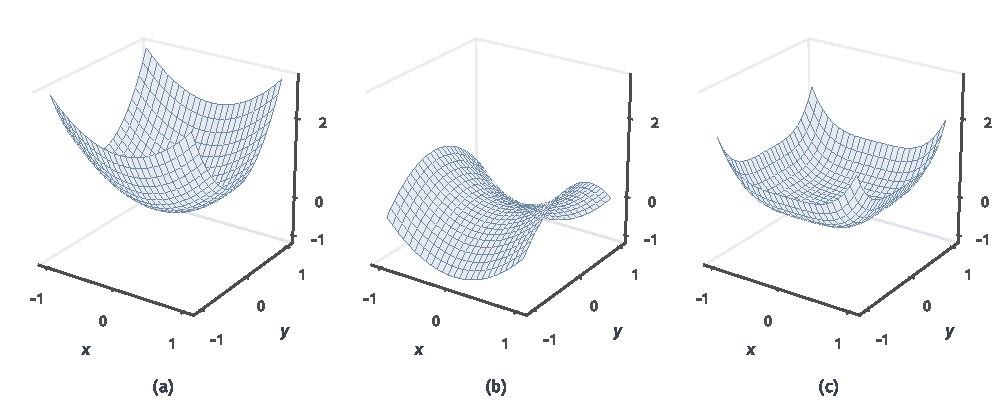
\includegraphics[width=169.0mm]{figures/00-shared/mathematical-preliminaries-upper/00-shared/matplotlib/chapter3-concept-processes/hessian-local-shapes.pdf}
 \caption{同一$[-1,1]^2$范围和纵轴尺度下，三面分别为$x^2+2y^2$、$x^2-y^2$、$x^4+y^4$。原点的Hessian依次为正定、不定、零矩阵；前两者给严格极小与鞍点，第三者虽严格极小却不能由正定判据推出。零Hessian也可能没有极值，例如前述$x^3$，故退化不是一种确定分类。}
 \label{fig:analysis-process-hessian-local-shapes}
\end{figure*}

